\documentclass{beamer}
\usepackage{graphicx,times}
\usepackage{natbib}        % required for bibliography
\usepackage{color}

\usepackage[utf8x]{inputenc}
\usepackage{lmodern,textcomp}
\usepackage{multirow}
%\usepackage{subfig}
%\usepackage{caption}
\usepackage{tipa}
\usepackage{graphicx}
\usepackage{hyperref}
\usepackage{multirow}
\usepackage{verbatim}
\usepackage{booktabs}
\usepackage{booktabs,siunitx}
\usepackage{amsmath}
\usepackage[export]{adjustbox}


\usepackage{graphicx,times}
\usepackage{natbib}        % required for bibliography
\usepackage{color}
\usepackage{mathtools}
\usepackage[english]{babel}
\usepackage[utf8x]{inputenc}
\usepackage{xcolor}
\usepackage{listings}



\usetheme{Boadilla}

%% Things to appear in the title page
\title{Resilience in Energy Management System}
\subtitle{A study case}
\author{Jesse J.\textsc{ PRINCE A.}}
\institute{IETR/CentraleSupelec}
\date{\today}

\begin{document}

%Page1
\begin{frame}
\titlepage
\end{frame}


%page4
\begin{frame}
\frametitle{Energy Management System}
\begin{itemize}
    \item What is an Energy Management System (EMS)  \vspace{10px}
    %Deja je ne suis pas dacord pr cette expression ou appelation de système car le EMS est simplement un controllerur qui lors de sa conception prend en compte des critères et contraines associés a des variables d"énergie
    \item Atype of EMS called HEMS \vspace{10px}
    \item EMS are classified in 3 families
    \item Many HEMS but few  tackle the presence of Grid Power Outage which is and example of Rare and Extreme event.
\end{itemize}
     
\end{frame}



%page4
\begin{frame}
\frametitle{Introduction}
What does existing HEMS propose when a GPO occurs ?
\pause
\begin{figure}[!ht]
    \begin{center}
        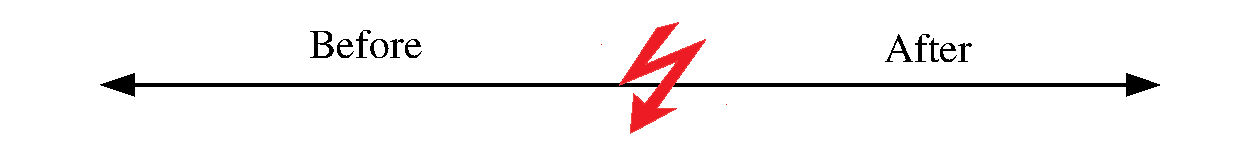
\includegraphics[width=1\columnwidth]{Figures/BefAfterGPO.pdf}
    \end{center}
\end{figure}
\pause
\vspace{-20px}
\begin{table}[]
\begin{tabular}{@{}c|c@{}}
\toprule
Do nothing \hspace{50px}& Switch to degrade mode \\ \midrule
\pause \multirow{2}{*}{\begin{tabular}[c]{@{}c@{}}Reserve always a constant \\ capacity of the battery\end{tabular}} & Do nothing \\ \cmidrule(l){2-2} 
 & Switch to degraded mode \\ \midrule
\pause \begin{tabular}[c]{@{}c@{}}Reserve smartly a variable capacity \\ of the battery\end{tabular} & \begin{tabular}[c]{@{}c@{}}Smartly switch between doing no-\\ thing and a variable degraded mode\end{tabular} \\ \bottomrule
\end{tabular}
\end{table}

\vspace{10px}
\pause Previous strategy consider a deterministic model of the GPO, In this work we propos to design a strategy using a \textbf{stochastic}  model of the GPO
\end{frame}


\begin{frame}
\frametitle{Outline}
\tableofcontents
\end{frame}

\section{Case study: Solar home}
\subsection{System Description}
\begingroup
\fontsize{10}{11}\selectfont
\begin{frame}

\frametitle{Case study: Solar home}

\begin{columns}
    \begin{column}{0.45\textwidth} 
        \pause \textbf{ External known variables}
        \begin{itemize}
            \item $P_{l}^*$: Home desired load profile;
            \vspace{3px} 
            \pause \item $P_{pv}^{max}$: Solar Panels Potential;
            \vspace{3px} 
            \pause \item $P_{g}^{max}$: Maximum electric grid power subscribed  by the user;
            
        \end{itemize} 
        \vspace{7px} 
        \pause \textbf{Decision variables}
        \begin{itemize}
            \item $P_{g}$: Power drawn from Grid \\
                \qquad $0 \leq P_{g} \leq P_{g}^{max}$
                \vspace{2px} 
            \pause \item $P_{curt}$:  Solar Curtailment \\ 
                \qquad $0 \leq P_{sp} \leq P_{pv}^{max}$ \quad \hspace{5px}
                \vspace{2px} 
            \pause \item $P_{s}$:  Load shedding \\
                \qquad $0 \leq P_{s} \leq P_{l}^*$ \quad 
                \vspace{2px} 
            \pause \item $P_{b}$:  Power in/out storage
        \end{itemize}
       \end{column}
\onslide<1->
    
    \begin{column}{0.55\textwidth}
        \begin{figure}[!ht]
            \begin{center}
                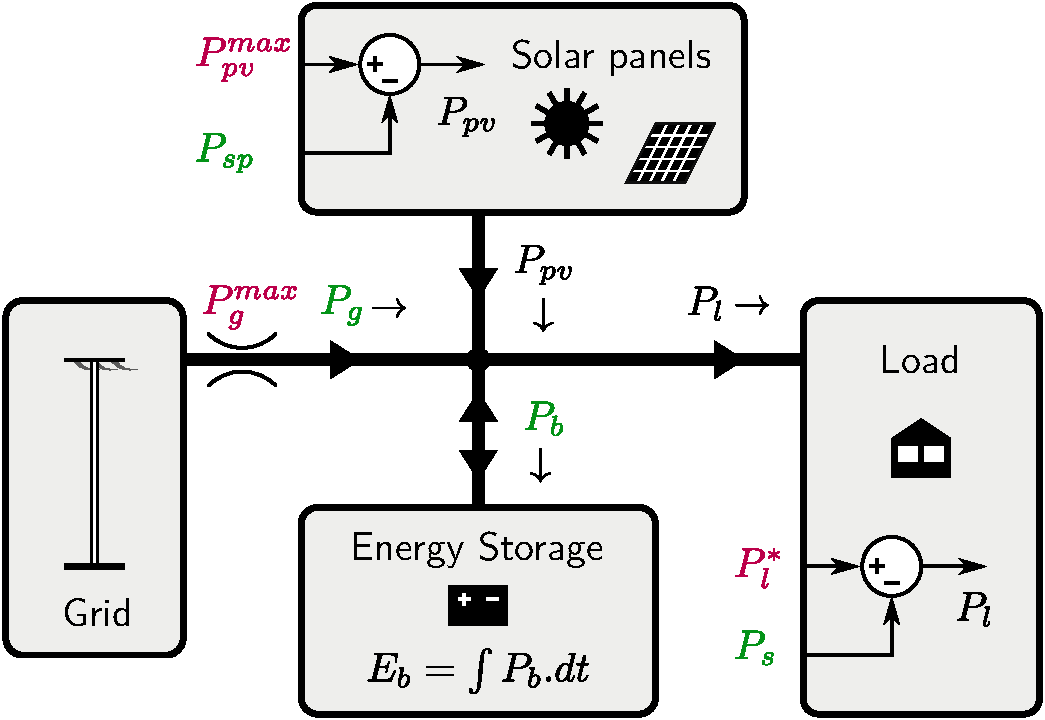
\includegraphics[width=1\columnwidth]{Figures/solar_home_compact.pdf}
            \end{center}
        \end{figure}
    \end{column}
\end{columns}

\vspace{5px}  
\pause \textbf{Storage dynamics:} $ E_{b}(k+1) = E_{b}(k) + P_{sto}(k)\Delta_t$ \\\vspace{5px}
\textbf{Storage constraint: }$0 \leq E_{b} \leq E_{rated}$ \\ \vspace{5px}

\end{frame}
\endgroup


\begingroup



\begingroup
\section{Towards the OLFC}
\subsection{Problem statement}
\fontsize{10}{11}\selectfont

\begin{frame}
\frametitle{Problem statement}
{\large Previous cited variable are all deterministic};
\vspace{15px}

{\large Stochastic availability of the Grid}  \\
\vspace{7px}
\begin{itemize}
    \item $P_g^{max}$ is a r.v, $P_g^{max} \in \mathcal{P}$
    \item $\mathcal{P}$ defined as $ \mathcal{P} = \left \{ P_0 , P_1\right \}$
\end{itemize}

\vspace{15px}
{\large Note that }
\begin{itemize}
    \item $P_0 = 0$ 
    \item $P_1$ is the maximum power subscribed by the user
\end{itemize}

\vspace{15px}
{\large When}
\begin{itemize}
\item $P_g^{max} = P_0 \rightarrow$ the grid is not available, an outage is occurring ; 
\item $P_g^{max} = P_1 \rightarrow$ the grid is available and we can draw energy from it . 
\end{itemize}
\end{frame}
\endgroup

\subsection{Deterministic controllers objectives}
\begin{frame}
\frametitle{Deterministic controllers objectives}
\vspace{15px}
{\Large Recall the main objectives}
\vspace{-15px}


    \pause

        \vspace{15px}
        \begin{itemize}
            \item \textbf{Obj A:} Minimize Electricity bill 
            \vspace{px}
            $$min\,C_{GRID} = \sum_{k=1}^{n} C_{grid}(k)P_{grid}(k)$$\\ 
            \vspace{-7px} $C_{grid}(k)$: Energy cost at time \textit{k}
            
            \vspace{26px}\pause 
             \item \textbf{Obj B:} Ensure the nominal comfort, $P_{load} = P_{load}^*$
             $$P_{load} = P_{load}^* - P_{shed}$$ \vspace{-15px}
             $$min\,P_{SHED} = \sum_{k=1}^{n} P_{shed}(k)$$ 
    
    
            \item \textbf{Obj C:} Ensure at least a degraded comfort ($P_{cri}$) during GPO, $P_{load} \geq P_{cri}$ 
            $$P_{load} \geq P_{cri}- P_{shed}^{\,cri}$$ \vspace{-15px}
             $$min\,P_{SHED}^{\,CRI} = \sum_{k=1}^{n} P_{shed}^{\,cri}(k)$$ 
        \end{itemize}

\end{frame}
\endgroup




%page 8
\begingroup
\fontsize{10}{11}\selectfont
\begin{frame}
\frametitle{Multi-objectives optimization}
\textbf{How to solve Multi-objectives optimization:}  
\begin{itemize}
    \item Convert Multi-objectives optimization into single objective;
    \item Linear scalarization: Aggregated with positive weights \\the sub-objectives functions to assign priority.
\end{itemize} \vspace{8px}

\textbf{Setting priority}
\begin{itemize}
    \item First : Satisfy degraded comfort (Obj C)
    \item Second : Satisfy nominal comfort (Obj B)
    \item Third : Minimize electricity bill (Obj A)
\end{itemize}\vspace{8px}

\end{frame}
\endgroup

\begin{frame}
\frametitle{Controller global objective}
\vspace{-10px}\textbf{RMPC global objective} \vspace{-10px}
%problème global en faisant une somme pondérée des couts associés aux objectifs ABC 
$$min \,J_{res} = \sum_{k=1}^{n} C_{grid}(k)P_{grid}(k) + C_s P_{shed}(k) + C_s^c P_{shed}^{cri}(k)$$

%Afin de montrer la priorité assicié a chque objectif la pondération .. de l'objectif C est trè trè supérieur
\textbf{$\forall k \in [1, n]$,} $C_s^c  \gg  Cs \gg max (C_{grid})$\\\vspace{12px}

\pause 
\textbf{MPC Framework}\\
\quad\textbf{H: }Prediction Horizon
\vspace{-5px}
$$J_{res}(k) = \sum_{i=k}^{k+H} C_{grid}(i)P_{grid}(i) + C_s P_{shed}(i) + C_s^c P_{shed}^{cri}(i),\, \forall \, k \in [1, n] $$ \\
\vspace{-7px}\hspace{11.6mm}$U_{k} = arg\,\underset{U_k}{\text{min}}\,J_{res}(k)$\\
\hspace{49px}= $(\textcolor{red}{u_{k|k}}, u_{k+1|k},\ldots,u_{k+H-1|k})$\\\vspace{10px}
\pause
\hspace{4px}with $\textcolor{red}{u_{k|k}}$ = [$P_{grid}(k);P_{curt}(k);P_{sto}(k);P_{shed};P_{shed}^{\,cri}(k)$]


\end{frame}



%page 10 
\begingroup
\fontsize{10}{11}\selectfont
\begin{frame}
\frametitle{Simulation}
\section{Simulation and results analysis}
\subsection{Simulation settings}
\begin{columns}
    \begin{column} {0.35\textwidth}
        {\Large Simulation settings}
        \begin{itemize}
        \vspace{4pt}
            \item Simulation over 3 day;
            \vspace{3pt}
            \item Simulation sample time $\Delta t = 0.5H$;
            \vspace{3pt}
            \item MPC prediction horizon H = 24H;
            \vspace{3pt}
            \item $P_{grid}^{max}=3kW$ and 0 during GPO
            \end{itemize}
    \end{column}
    
    \begin{column}{0.65\textwidth}
                 
        \begin{figure}[!ht]
        \begin{center}
                \includegraphics[width=1\columnwidth]{Figures/confFig2.pdf}
        \end{center}
        %\caption{Power flow model of a solar home}
        \label{Config1}
\end{figure}
        
    \end{column}
\end{columns}

\begin{itemize}
    \item  $C_{grid}$ consist of two energy price 
        \begin{itemize}
            \item $C_{night}$: Off-peak hour, from 12:00 a.m. to 6:00 a.m
            \item $C_{day}$: On-peak hour from 6:30 a.m. to 23:30 p.m
        \end{itemize}
    \item The GPO occurs at 00h30 a.m. the second day; 
    \item $P_{cri} = 0.5P_{load}^*$
    \item $E_{rated} $= 8kWh
    
\end{itemize}



\end{frame}
\endgroup



%page 12 
\begin{frame}
\frametitle{Other controllers}
\textbf{Classic controller:} Satisfy obj A et Obj B.
\vspace{10pt}

\textbf{Rule based controller power save with reserve:} (RBCPS-R):Compute $P_{nl} = P_{sun}$ - $P_{load}^*$. If $P_{nl}>0$, store the excessive energy into storage, otherwise use grid and storage to sustain house demand\begin{itemize}
    \item Nominal mode: $E_{sto}\geq E_{sto}^{res} $
    \item Degraded mode: \begin{itemize}
        \item $P_{load} = P_{cri}$
        \item $E_{sto}\geq 0 $
    \end{itemize}
\end{itemize}
\end{frame}




%page 14
\begin{frame}{Comfort satisfaction indexes}



\begin{columns}

    \begin{column}{0.3\textwidth}
    \begin{center}
    The load satisfaction level\\\vspace{12px}
            Bad: $L{c-}$\\ \vspace{6px}
            Good: $L_{c+}$\\\vspace{6px}
            Perfect: $L^*$
        \end{center}
        
    \end{column}
    \begin{column}{0.4\textwidth}
        \begin{center}
           The load satisfaction ratio  $\lambda = \frac{P_{load}}{P_{load}^*}$\\ \vspace{10px}
            $0 \leq \lambda<\lambda_{cri}$ \quad\qquad or \\ \vspace{6px}
            $\lambda_{cri}\leq \lambda < 1$ \quad\qquad  or \\\vspace{6px}
            $\lambda=1$ \hspace{65px}or 
        \end{center}
        
    \end{column}
    
    \begin{column}{0.35\textwidth}
    \vspace{40px}
    \begin{center}
            $0\leq P_{load}<P_{cri}$\\ \vspace{5px}
            $P_{cri}\leq P_{load}<P_{load}^*$\\\vspace{5px}
            $P_{load}=P_{load}^*$
        \end{center}
        
    \end{column}
    
\end{columns}

\begin{figure}[!ht]
        \begin{center}
                \includegraphics[width=0.7\columnwidth]{Figures/load_satisfaction_intervals.pdf}
        \end{center}
        \end{figure}
    
    
\end{frame}

        

%page 14 
\begin{frame}
\frametitle{Class VS RMPC PV4 Scheduled GPO}
\subsection{Result Analysis}

\begin{figure}[!ht]
        \begin{center}
                \includegraphics[width=1\columnwidth]{Figures/ScheduleData.pdf}
        \end{center}
        \end{figure}
\end{frame}


\begin{frame}
\frametitle{RBCPSR VS RMPC PV4 Unscheduled GPO}

\end{frame}



%page 15 
\begingroup
\fontsize{9}{11}\selectfont
\begin{frame}
\frametitle{Sheduled and Unscheduled table}


    \begin{table}[!ht]
        \renewcommand{\arraystretch}{1.1}
        %\caption{Class VS RMPC performances : Scheduled GPO}
        \centering

        \begin{center}
            \begin{tabular}{lcc||*{4}{c|}c||}
		 \cline{4-8}
		 
	            \multirow{2}{*}{} & \multirow{2}{*}{}
        	    &\multirow{2}{*}{} &\multirow{2}{*}{$P_{grid}$} & \multirow{2}{*}{$P_{curt}$}
	            &\multicolumn{3}{c||}{\begin{tabular}[c]{@{}c@{}}Time spent at the load\\ satisfaction level during \\the GPO (in \%)\end{tabular}}\\ \cline{2-3}\cline{6-8}
	            & Scenario & Controller &  &  & $L_{c-}$ & $L_{c+}$ & $L^*$\\
	            \cmidrule[1pt]{1-8} 
	
                \parbox[t]{1.5mm}{\multirow{4}{*}{\rotatebox[origin=c]{90}{Sched GPO}}} &\multirow{2}{*}{PV2} &Class   &\multirow{2}{*}{14} &\multirow{2}{*}{0} &\textcolor{red}{\textbf{32.3}} &3.1 &64.6 \\ \cline{3-3}
                & & RMPC  &  &     &\textcolor{green}{\textbf{0}}   &62.5  &37.5\\ \cmidrule[1pt]{2-8} 
                     
                &\multirow{2}{*}{PV4} &Class   &\multirow{2}{*}{4.8} &\multirow{2}{*}{4.5} &\textcolor{red}{\textbf{15.6}} &1 &83.4 \\ \cline{3-3}
                & &RMPC  &  &     &\textcolor{green}{\textbf{0}}   &25.2  &74.8\\ \hline \cmidrule[1pt]{1-8}
                \pause
                
                \parbox[t]{1.5mm}{\multirow{4}{*}{\rotatebox[origin=c]{90}{Unsch GPO}}}
                &\multirow{2}{*}{PV2} &RBCPS 20\%   &7.6 &\multirow{2}{*}{0} &\textcolor{green}{\textbf{27.7}} &72.3 &0 \\ \cline{3-3}
                & & RMPC & 7.2 &  &\textcolor{red}{\textbf{28.1}} & 58.3 &13.6\\ \cmidrule[1pt]{2-8} 
                
                & \multirow{2}{*}{PV4} &RBCPS 20\%   &1.8 &12.8 &\textcolor{green}{\textbf{0}} &100 &0 \\ \cline{3-3}
                & & RMPC &1.5 &4.5 &\textcolor{green}{\textbf{0}}  &40.6 &59.4\\ \cmidrule[1pt]{1-8} 
    
            \end{tabular}
        \end{center}
\end{table}
Unschedulled GPO : Lower performances 

\end{frame}
\endgroup


\section{Conclusion \& Future Work}

%page 16
\begin{frame}
\frametitle{Conclusion \& Future Work}
\textbf{Conclusion:} We have developed a flexible Controller which in case of an REE adapts to the situation without changing its global objectives \\
\vspace{30pt}
\textbf{Future work:} Integrate the uncertain character on an RE into the controller

\end{frame}


%\page 18
\begin{frame}
\frametitle{}
        \begin{center}
{\Large THANK YOU FOR YOUR ATTENTION}

\begin{figure}[!ht]

                \includegraphics[width=0.6\columnwidth]{Figures/endPict.pdf}
                
        
\end{figure}
\end{center}

\end{frame}


\end{document}